\documentclass[
  captions=tableheading,
  bibliography=totoc, 
  titepage=firstiscover,
]{scrartcl}

\usepackage{blindtext} %neuer input

\usepackage{longtable} % Tabellen über mehrere Seiten

\usepackage[utf8]{inputenc} %neuer input

\usepackage{scrhack}

\usepackage[aux]{rerunfilecheck} %Warnung falls nochmal kompiliert werden muss

\usepackage{fontspec} %Fonteinstellungen

\recalctypearea{}

\usepackage[main=ngerman]{babel} %deutsche Spracheinstellung

\usepackage{ragged2e} %neuer input

\usepackage{amsmath, nccmath}

\usepackage{amssymb} %viele mathe Symbole

\usepackage{mathtools} %Erweiterungen für amsmath


\DeclarePairedDelimiter{\abs}{\lvert}{\rvert}
\DeclarePairedDelimiter{\norm}{\lVert}{\rVert}

\DeclarePairedDelimiter{\bra}{\langle}{\rvert}
\DeclarePairedDelimiter{\ket}{\lvert}{\rangle}

\DeclarePairedDelimiterX{\braket}[2]{\langle}{\rangle}{
#1 \delimsize| #2
}

\NewDocumentCommand \dif {m}
{
\mathinner{\symup{d} #1}
}


\usepackage[
  math-style=ISO,
  bold-style=ISO,
  sans-style=italic,
  nabla=upright,
  partial=upright,
  warnings-off={
    mathtools-colon,
    mathtools-overbracket,
  },
]{unicode-math}

\setmathfont{Latin Modern Math}
\setmathfont{XITS Math}[range={scr, bfscr}]
\setmathfont{XITS Math}[range={cal, bfcal}, StylisticSet=1]


\usepackage[
  locale=DE,
  separate-uncertainty=true,
  per-mode=reciprocal,
  output-decimal-marker={,},
]{siunitx}

\usepackage[autostyle]{csquotes} %richtige Anführungszeichen

\usepackage{xfrac}

\usepackage{float}

\floatplacement{figure}{htbp}

\floatplacement{table}{htbp}

\usepackage[ %floats innerhalb einer section halten
  section,   %floats innerhalb er section halten
  below,     %unterhalb der Section aber auf der selben Seite ist ok
]{placeins}

\usepackage[
  labelfont=bf,
  font=small,
  width=0.9\textwidth,
]{caption}

\usepackage{subcaption} %subfigure, subtable, subref

\usepackage{graphicx}

\usepackage{grffile}

\usepackage{booktabs}

\usepackage{microtype} %Verbesserungen am Schriftbild

\usepackage[
backend=biber,
]{biblatex}

\addbibresource{../lit.bib}

\usepackage[ %Hyperlinks im Dokument
  german,
  unicode,
  pdfusetitle,
  pdfcreator={},
  pdfproducer={},
]{hyperref}

\usepackage{bookmark}

\usepackage[shortcuts]{extdash}

%\usepackage{warpcol}

\usepackage{physics}
\allowdisplaybreaks

\begin{document}
    \title{Physik IV Übungsblatt 11}
    \author{  
    Tobias Rücker\\
    \texorpdfstring{\href{mailto:tobias.ruecker@tu-dortmund.de}{tobias.ruecker@tu-dortmund.de}
    \and}{,} 
    Paul Störbrock\\
    \texorpdfstring{\href{mailto:paul.stoerbrock@tu-dortmund.de}{paul.stoerbrock@tu-dortmund.de}}{}
    }
\maketitle
\center{\Large Abgabegruppe: \textbf{4H}}
\thispagestyle{empty}

\newpage
\tableofcontents
\thispagestyle{empty}
\newpage

\setcounter{page}{1}

\section{Aufgabe 1}
\begin{figure}[H]
    \centering
    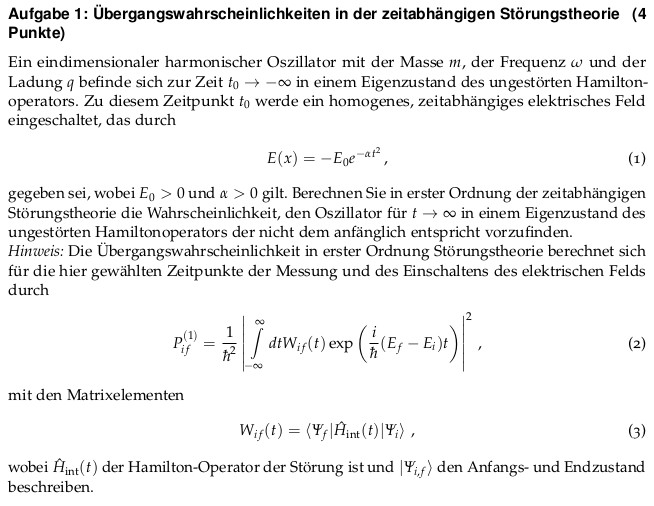
\includegraphics[width=\textwidth]{images/ex1.jpg}
\end{figure}
Bestimmung des Störungsteil des Hamilton-Operator:
\begin{align}
    q E(t,x) &= - \del{}{x} \phi \\
    \phi &= \int q E_0 e^{- \alpha t^2} \,\dif{x}\\
    &=q E_0 x e^{-\alpha t^2}\\
    \hat H _{int} (t) &= q E_0 \hat x e^{-\alpha t^2}\\
    \intertext{
        Bestimmung der Matrixelemente $W_{if}(t) $
    }
    \bra{\psi _f} q E_0 \hat x e^{- \alpha t^2} \ket{\psi _i}&= q E_0 e^{-\alpha t^2} \bra{\psi _f} \hat x \ket{\psi _i}  \\
    \intertext{
        Um die Wahrscheinlichkeit von einem Zustand i in einen beliebigen Zustand f
        zu bestimmen, wird die Formel 2 vom Blatt über alle f summiert.
    }
    \sum _{f, f \ne i} P_{if}^{(1)} &= \sum _{f, f \ne i} \frac{1}{\hbar ^2} \abs{ \int_{-\infty}^{\infty} \.\dif{t} q E_0 e^{-\alpha t^2} \bra{\psi _f} \hat x \ket{\psi _i} \exp \left( \frac{i}{\hbar} (E_f - E_i)t \right) }^2\\
    \intertext{
        Zwischenrechnung:
    }
    \hat x &= \sqrt{\frac{\hbar}{2m \omega}} (\hat a + \hat a ^\dagger)\\
    \bra{\psi _f} \sqrt{\frac{\hbar}{2m \omega}} (\hat a + \hat a ^\dagger) \ket{\psi _i}\\
    &= \sqrt{\frac{\hbar}{2m \omega}} (\bra{\psi _f} \hat a \ket{\psi _i} + \bra{\psi _f} \hat a ^{\dagger} \ket{\psi _i} )\\
    &= \sqrt{\frac{\hbar}{2m \omega}} (\sqrt{i} \delta _{f,i-1} + \sqrt{i+1} \delta _{f,i+1} )\\
    \intertext{
        Einsetzen in P und weiterrechnen
    }
    &= \sum _{f, f \ne i} \frac{1}{\hbar ^2} \abs{ \int_{-\infty}^{\infty} \,\dif{t} q E_0 \sqrt{\frac{\hbar}{2m \omega}} e^{-\alpha t^2} \exp \left( \frac{i}{\hbar} (E_f-E_i)t \right) (\sqrt{i} \delta _{f,i-1} + \sqrt{i+1} \delta _{f,i+1} ) }^2  \\
    &= \sum _{f, f \ne i} \frac{q^2 E_0^2}{2 \hbar m \omega}  \abs{\sqrt{i} \delta _{f,i-1} + \sqrt{i+1} \delta _{f,i+1} }^2 \abs{ \int_{-\infty}^{\infty} \,\dif{t} \exp \left(-\alpha t^2 \frac{i}{\hbar} (E_f-E_i)t \right)  }\\
    \intertext{
        quadratische Ergänzung und Substitution des Exponenten zum Lösen des Integrals
    }
    - \alpha t^2 + \underbrace{\frac{i}{\hbar} (E_f -E_i) }_{=C} t\\
    &= - \alpha \left(t^2 - \frac{C}{\alpha} t + \frac{C^2}{4\alpha ^2} - \frac{C^2}{4 \alpha ^2} \right)\\
    &= - \alpha \left( t- \frac{C}{2 \alpha} \right)^2 + \frac{C^2}{4 \alpha}\\
    u  &= t-\frac{C}{2 \alpha}\\
    \frac{\dif{u}}{\dif{t}}=1\\
    \intertext{weiter mit der Rechnung}
    &= \sum _{f, f \ne i} \frac{q^2 E_0^2}{2 \hbar m \omega} \abs{\sqrt{i} \delta _{f,i-1} + \sqrt{i+1} \delta _{f,i+1} }^2 \abs{\int_{-\infty}^{\infty} \,\dif{u} e^{\frac{c^2}{4\alpha} \exp (-\alpha u^2) } }^2\\
    &= \sum _{f, f \ne i} \frac{q^2 E_0^2}{2 \hbar m \omega} e^{\frac{C^2}{2\alpha}} \abs{\sqrt{i} \delta _{f,i-1} + \sqrt{i+1} \delta _{f,i+1} }^2 \abs{\sqrt{\frac{\pi}{\alpha}}}^2\\
    \intertext{
        Beim Auflösen der Summe bleiben nur die Elemente mit $f=i\pm 1$ übrig. Alle
        anderen verschwinden. Für $C^2$ ergibt sich dadurch.
    }
    C^2 &= -\frac{1}{\hbar ^2} (E_{i\pm 1} - E_i)^2 \\
    &= -\frac{1}{\hbar ^2} (i\pm 1 + \frac{1}{2}-i-\frac{1}{2} )^2 \hbar ^2 \omega ^2\\
    &= -\omega ^2\\
    \intertext{weiter}
    &= \frac{q^2 E_0^2 \pi}{2 \hbar m \omega \alpha} \exp \left(\frac{- \omega ^2}{2\alpha}\right) (2i+1)
\end{align}

\section{Aufgabe 2}
\begin{figure}[H]
    \centering
    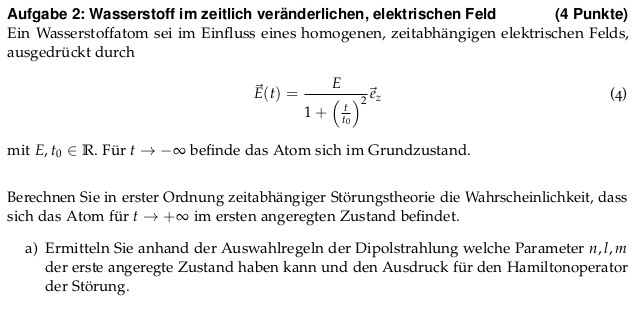
\includegraphics[width=\textwidth]{images/ex2a.jpg}
\end{figure}
\begin{figure}[H]
    \centering
    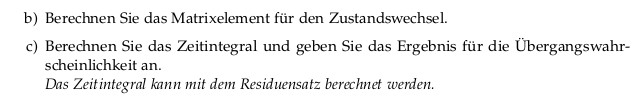
\includegraphics[width=\textwidth]{images/ex2b.jpg}
\end{figure}
\subsection{a)}


\subsection{b)}


\subsection{c)}


\section{Aufgabe 3}
\begin{figure}[H]
    \centering
    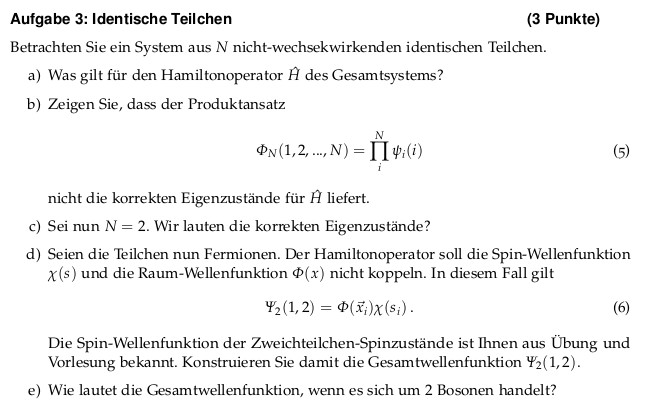
\includegraphics[width=\textwidth]{images/ex3.jpg}
\end{figure}
\subsection{a)}


\subsection{b)}


\subsection{c)}


\subsection{d)}


\subsection{e)}


\section{Aufgabe 4}
\begin{figure}[H]
    \centering
    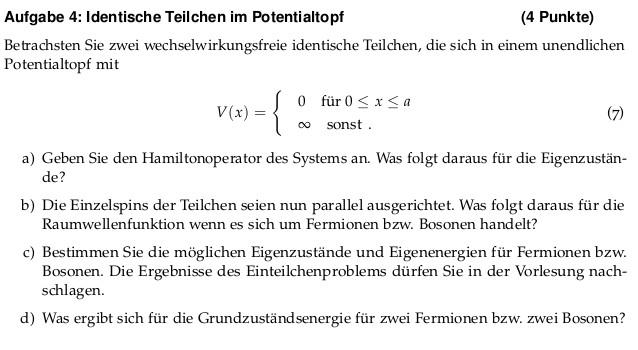
\includegraphics[width=\textwidth]{images/ex4.jpg}
\end{figure}

\subsection{a)}

\subsection{b)}

\subsection{c)}

\subsection{d)}


\end{document}